\section{GW}

\begin{frame}
    \frametitle{Introduction}
    The Dyson equation is
\begin{equation}
    G = G_0 + G_0 \Sigma G
\end{equation}
where $G$ is the interacting Green's function, $G_0$ is the non-interacting Green's function, and $\Sigma= iGW\Gamma $ is the proper self-energy.
\pause
The $GW$ approximation for the self-energy is

\begin{align}
    \Sigma
    &\approx iGW
\end{align}

\end{frame}
\begin{frame}
    \frametitle{Hedin's Equations \cite{article}}
 \begin{figure}
    \centering
    \includegraphics[width=0.5\textwidth]{figs/hedin_pentagon.png}
 \end{figure}

\end{frame}

\begin{frame}
    \frametitle{Frequency Integral \cite{Zhu2020-nt}}
\begin{align}
    \Sigma ^{GW}(\mathbf{r}, \mathbf{r}^{\prime} ; \omega)&=\frac{i}{2 \pi} \int_{-\infty}^{\infty} d \omega^{\prime} G\left(\mathbf{r}, \mathbf{r}^{\prime} ; \omega+\omega^{\prime}\right) W\left(\mathbf{r}, \mathbf{r}^{\prime} ; \omega^{\prime}\right) \\
&\equiv \Sigma ^x(\mathbf{r}, \mathbf{r}^{\prime}) + \color{red}{\Sigma ^{c}(\mathbf{r}, \mathbf{r}^{\prime} ; \omega)}
\end{align}
\pause
where the exact expression for the correlation self-energy is
\begin{align}
    \color{red}\Sigma_{pq}^{c}(\omega) &= \sum_{\mu }^{\text{RPA}}\left(\sum_{i}^{\text{O}} \frac{w_{pi}^{\mu }w_{iq}^{\mu }}{\omega -(\epsilon _{i}-\Omega  _{\mu })+i\eta}+ \sum_{a}^{\text{V}} \frac{w_{pa}^{\mu }w_{aq}^{\mu }}{\omega -(\epsilon _{a}+\Omega  _{\mu })-i\eta}\right)
\end{align}
\pause
To get the $\Omega _{\mu }$ and $w_{pq}^{\mu }$, we solve the RPA eigenvalue problem, which scales as $O(N^6)$.
\end{frame}

\begin{frame}
    \frametitle{How does this expression come about?}
\begin{figure}
    \centering
    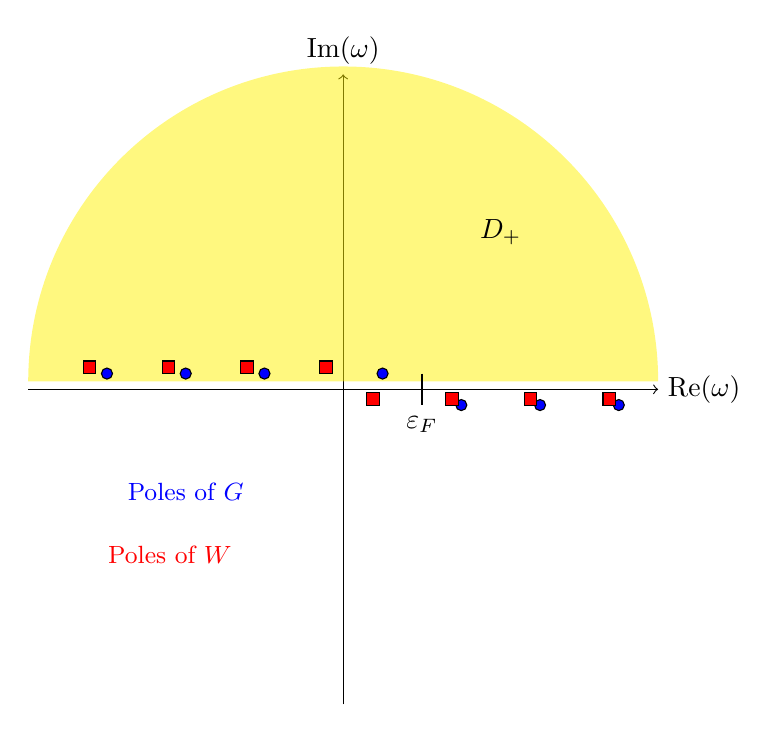
\begin{tikzpicture}
    % Draw the axes
    \draw[->] (-4, 0) -- (4, 0) node[right] {Re($\omega$)};
    \draw[->] (0, -4) -- (0, 4) node[above] {Im($\omega$)};
    


    % Draw the semicircle contours
    % fill in its under side
    \fill[yellow, opacity=0.5] (4, 0.1) arc[start angle=0, end angle=180, radius=4];
    % \fill[red, opacity=0.3] (4, -0.1) arc[start angle=0, end angle=-180, radius=4];
    

    % --- Fermi energy marker ---
    \draw[thick] (1, 0.2) -- (1, -0.2);
    \node at (1, -0.45) {$\varepsilon_{F}$};

    % --- Poles of G (blue circles) ---
    % Above the real axis (occupied states)
    \foreach \x in {-3,-2,-1,0.5} {
        \draw[fill=blue] (\x, 0.2) circle (2pt);
    }

    % Below the real axis (unoccupied states)
    \foreach \x in {1.5,2.5,3.5} {
        \draw[fill=blue] (\x, -0.2) circle (2pt);
    }

    % Label for poles of G
    \node[text=blue] at (-2, -1.3) {\small Poles of $G$};

    % --- Poles of W (red squares, not rotated, slightly offset) ---
    % Above the real axis for negative Re(ω)
    \foreach \x in {-3.3,-2.3,-1.3, -0.3} {
        \draw[fill=red] (\x, 0.2) rectangle ++(0.16,0.16);
    }

    % Below the real axis for positive Re(ω)
    \foreach \x in {0.3, 1.3,2.3,3.3} {
        \draw[fill=red] (\x, -0.2) rectangle ++(0.16,0.16);
    }

    % Label for poles of W
    \node[text=red] at (-2.2, -2.1) {\small Poles of $W$};

    
    % Label the contours
    \node at (2, 2) {$D_+$};
    % \node at (-2, -2) {$D_-$};
\end{tikzpicture}
\end{figure}

\end{frame}

\begin{frame}
    \frametitle{Analytic continuation: the plot}
\begin{figure}
    \centering
    \begin{tikzpicture}[scale=1.1]

    % --- Axes ---
    \draw[->, thick] (-4, 0) -- (4, 0) node[right] {Re($\omega$)};
    \draw[line width=3pt] (0, -3.5) -- (0, 3.5) node[above] {Im($\omega$)};


    % --- Fermi energy marker ---
    \draw[thick] (1, 0.2) -- (1, -0.2);
    \node at (1, -0.45) {$\varepsilon_{F}$};

    % --- Poles of G (blue circles) ---
    % Above the real axis (occupied states)
    \foreach \x in {-3,-2,-1,0.5} {
        \draw[fill=blue] (\x, 0.2) circle (2pt);
    }

    % Below the real axis (unoccupied states)
    \foreach \x in {1.5,2.5,3.5} {
        \draw[fill=blue] (\x, -0.2) circle (2pt);
    }

    % Label for poles of G
    \node[text=blue] at (-2, -1.3) {\small Poles of $G$};

    % --- Poles of W (red squares, not rotated, slightly offset) ---
    % Above the real axis for negative Re(ω)
    \foreach \x in {-3.3,-2.3,-1.3, -0.5} {
        \draw[fill=red] (\x, 0.2) rectangle ++(0.16,0.16);
    }

    % Below the real axis for positive Re(ω)
    \foreach \x in {0.3, 1.3,2.3,3.3} {
        \draw[fill=red] (\x, -0.2) rectangle ++(0.16,0.16);
    }

    % Label for poles of W
    \node[text=red] at (-2.2, -2.1) {\small Poles of $W$};

    \end{tikzpicture}
\end{figure}



\end{frame}

\begin{frame}
    \frametitle{Analytic continuation: the equations}
    Perform
\begin{equation}
    \Sigma ^{c}(\mathbf{r}, \mathbf{r}^{\prime}, i \omega) = -\frac{1}{2 \pi} \int_{-\infty}^{\infty} d \omega^{\prime} G\left(\mathbf{r}, \mathbf{r}^{\prime}, i \omega+i \omega^{\prime}\right) W\left(\mathbf{r}, \mathbf{r}^{\prime}, i \omega^{\prime}\right)
\end{equation}
\pause
and then analytically continue to real frequencies, obtaining $\Sigma ^{c}(\mathbf{r}, \mathbf{r}^{\prime} ; \omega)$.
\end{frame}
\begin{frame}
    \frametitle{Contour deformation: the plot}
\begin{figure}
    {\setlength{\fboxrule}{2pt}\setlength{\fboxsep}{3pt}% border thickness and padding
        \fcolorbox{red}{white}{\includegraphics[width=0.5\textwidth]{figs/gw_contour.jpeg}}%
    }
\end{figure}
\end{frame}
\begin{frame}
    \frametitle{Contour deformation: the equations}
Split into parts as
\begin{align}
    \color{red}{\oint \cdots} &= \color{green}{\int_{\operatorname{Re}} \cdots}\color{black}+\color{blue}{\int_{\operatorname{Im}} \cdots}\color{black}+\int_{\operatorname{arc} \Gamma^{+}} \cdots+\int_{\operatorname{arc} \Gamma^{-}} \cdots \\
\implies \color{green} {\int_{\operatorname{Re}} \cdots} &= \color{red}{\oint \cdots} \color{black}- \color{blue}{\int_{\operatorname{Im}} \cdots}
\end{align}
% $\begin{aligned} & \frac{i}{2 \pi} \oint d \omega^{\prime} G_0\left(\omega+\omega^{\prime}\right) W_0\left(\omega^{\prime}\right) \\ & \quad=\int_{\operatorname{Re}} \cdots+\int_{\operatorname{Im}} \cdots+\int_{\operatorname{arc} \Gamma^{+}} \cdots+\int_{\operatorname{arc} \Gamma^{-}} \cdots\end{aligned}$
% $\begin{aligned} \Sigma\left(\mathbf{r}, \mathbf{r}^{\prime}, \omega\right)= & \frac{i}{2 \pi} \oint d \omega^{\prime} G_0\left(\mathbf{r}, \mathbf{r}^{\prime}, \omega+\omega^{\prime}\right) W_0\left(\mathbf{r}, \mathbf{r}^{\prime}, \omega^{\prime}\right) \\ & -\frac{1}{2 \pi} \int_{-\infty}^{\infty} d \omega^{\prime} G_0\left(\mathbf{r}, \mathbf{r}^{\prime}, \omega+i \omega^{\prime}\right) W_0\left(\mathbf{r}, \mathbf{r}^{\prime}, i \omega^{\prime}\right)\end{aligned}$
\end{frame}
\begin{frame}
\frametitle{A summary of frequency integration schemes}
\begin{table}
    \centering
    \small
    \begin{tabular}{|c|c|c|}
    \hline
    \textbf{Method} & \textbf{Scaling} & \textbf{Comments} \\
    \hline
    \onslide<1->{Fully analytic & $O(N^6)$ & \parbox{4cm}{Evaluate the real frequency integral by integrating over a contour, which spans the positive imaginary axis.} \\ \hline}
    \onslide<2->{Analytic continuation & $O(N^4)$ & \parbox{4cm}{Avoid all poles by integrating along imaginary frequency axis, then analytically continuing to real frequencies.} \\ \hline}
    \onslide<3->{Contour deformation & $O(N^5)$ & \parbox{4cm}{Deform the contour to do the integral in a piecewise fashion.} \\ \hline}
    \onslide<4->{Frequency-free & $O(N^4)$ & \parbox{4cm}{Perform convolution without frequency dependence, so we are not constrained by the poles.} \\ \hline}
    \end{tabular}
\end{table}
\end{frame}



\begin{frame}
    \frametitle{Solving the quasi-particle (QP) equation}
In $GW$, we can compute QP energies by solving:
\begin{equation}
    \epsilon ^{QP}_p = \color{yellow}{\epsilon^{HF}_p} \color{black}+ \operatorname{Re}\left(\Sigma_{pq} ^c (\omega)\right)\delta_{pq}
\end{equation}
\pause
with
\begin{equation}
    \Sigma_{pq}^{c}(\omega) = \sum_{\mu }^{\text{RPA}}\left(\sum_{i}^{\text{occupied}} \frac{\color{purple}{w_{pi}^{\mu }w_{iq}^{\mu }}}{\color{red}{\omega -(\epsilon _{i}-\Omega  _{\mu })+i\eta}}+ \sum_{a}^{\text{virtual}} \frac{\color{green}{w_{pa}^{\mu }w_{aq}^{\mu }}}{\color{blue}{\omega -(\epsilon _{a}+\Omega  _{\mu })-i\eta}}\right)
\end{equation}
\pause
Using Lowdin partitioning we can recast this as a matrix problem
\begin{equation}
    \bm{H}^{GW} = \begin{pmatrix} \color{yellow}{\bm{F}} & \color{purple}{\bm{W}^<} & \color{green}{\bm{W}^>} \\ \color{purple}{\bm{W}^{<,\dagger}} & \color{red}{\bm{d}^<} & 0 \\ \color{green}{\bm{W}^{>, \dagger}} & 0 & \color{blue}{\bm{d}^>} \end{pmatrix}
\label{eq:booth_hamiltonian}
\end{equation}
\pause
The QP energies and Dyson orbitals are the eigenpairs of $\bm{H}^{GW}$.
\end{frame}

\begin{frame}
    \frametitle{Moment-conserving GW \cite{scott2023moment}}
\begin{enumerate}
    \item Devises a Lanczos procedure to iteratively diagonalize equation \ref{eq:booth_hamiltonian}.
    \pause
    \item I found that in the limit of a large number of Lanczos iterations, eigenvalues do not converge to the exact answer.
\end{enumerate}
\pause
\begin{figure}
    \centering
    \includegraphics[width=0.85\textwidth]{../images/mcgw_issues.png}
\end{figure}
\end{frame}

\begin{frame}
    \frametitle{Why?}
\begin{enumerate}
    \item A Krylov subspace is never explicitly constructed.
     \pause
    \item Therefore, it cannot be reorthogonalized, so there is no guarantee that the Ritz values will converge to the true eigenvalues.
\end{enumerate} 
\end{frame}

\section{Cumulant Expansion}


\begin{frame}
    \frametitle{The ansatz}
\begin{align}
    G(t) = G_0(t) e^{C(t)} = \color{red}{G_0(t) \left[1 + C(t) + \frac{C(t)^2}{2} + \ldots \right]}
\label{eq:cumulant_expansion}
\end{align}
\pause
vs.
\begin{align}
    G(t) = \color{red}{G_0(t) + G_0(t) \Sigma(t) G_0(t) + G_0(t) \Sigma(t) G_0(t) \Sigma(t) G_0(t) + \ldots }
\label{eq:dyson_expansion}
\end{align}
\pause
\begin{table}
    \centering
    \small
    \begin{tabular}{|c|c|}
    \hline
    \textbf{Perturbation series} & \textbf{Interpretation} \\
    \hline
    \onslide<1->{Equation \ref{eq:cumulant_expansion} & Treats all diagrams approximately \\ \hline}
    \onslide<2->{Equation \ref{eq:dyson_expansion} & Treats some diagrams exactly, and neglects others entirely. \\ \hline}
    \end{tabular}
\end{table}
    
\end{frame}

\begin{frame}
    \frametitle{What is done in popular cumulant schemes for electronic structure?}
\begin{itemize}
    \item Equate \ref{eq:cumulant_expansion} and \ref{eq:dyson_expansion} to low order in the interaction.
    \item Use a known form for the self-energy, most commonly the $GW$ form.
\end{itemize}
\pause
This leads to the famous Landau formula for the cumulant, which is
\begin{equation}
    C(t)=\int d \omega \frac{\beta(\omega)}{\omega^2}\left[e^{-i \omega t}+i \omega t-1\right]
\end{equation}
where the cumulant kernel is defined as
\begin{equation}
    \beta(\omega)=-\frac{1}{\pi} \operatorname{Im} \Sigma^{\mathrm{c}}(\omega)
\end{equation}
\end{frame}

\begin{frame}
    \frametitle{What hasn't been explored?}
\pause
\begin{enumerate}
    \item Studying UEG in a finite basis
    \pause
    \item Numerical self-consistency
    \pause
    \item Using second-order self-energy, instead of the $GW$ form
\end{enumerate}
\end{frame}
\begin{frame}
    \frametitle{Numerical self-consistency scheme}
We want
\begin{equation}
    G_{pp}^R(t) = -i \Theta(t) e^{-i \epsilon_p t} e^{C_{pp}^{(2)}(t)} 
\label{eq:sc_cumulant_greens_time}
\end{equation}
with 
\begin{align}
C_{pp}^{(2)}(t) &\equiv i \int \frac{d\omega}{2\pi} \frac{ {\Sigma}_{pp}^{c,(2)}\left(\omega+\epsilon_p\right)}{(\omega + i \eta)^2} e^{-i \omega t}
\end{align}
\pause
\begin{align}
&= \frac{1}{2}\sum_{iab} \frac{\left< pi \left| \right| ab \right>^2}{\left(\epsilon_{pi}^{ab}\right)^2}
\left(e^{-i \epsilon_{pi}^{ab} t} +i \epsilon_{pi}^{ab} t -1 \right) \label{eq:cumulant_2nd_final}\\
&+\frac{1}{2}\sum_{ija} \frac{\left< pa \left| \right| ij \right>^2}{\left(\epsilon_{pa}^{ij}\right)^2}
\left(e^{-i \epsilon_{pa}^{ij} t} +i \epsilon_{pa}^{ij} t -1 \right) \nonumber 
\end{align}
where
$\epsilon_{pi}^{ab} = \epsilon_{a}+\epsilon_{b}-\epsilon_{p}-\epsilon_{i}$
and
$\epsilon_{pa}^{ij} = \epsilon_{i}+\epsilon_{j}-\epsilon_{p}-\epsilon_{a}$.
\end{frame}
\begin{frame}
    \frametitle{Numerical self-consistency scheme (cont.)}
So, do:
\begin{enumerate}
    \item Start with HF orbital energies $\epsilon_p$ and coefficients $C_{\mu p}$.
    \pause
    \item Get $G_{pp}^R(t) = -i \Theta(t) e^{-i \epsilon_p t} e^{C_{pp}^{(2)}(t)}$ with $C_{pp}^{(2)}(t)$ from \ref{eq:cumulant_2nd_final}.
    \pause
    \item $G_{pp}^R(\omega) = \mathrm{FFT}\left[ G_{pp}^R(t) \right]$.
    \pause
    \item $A_{pp}(\omega) = -\frac{1}{\pi} \operatorname{Im}\left[ G_{pp}^R(\omega) \right]$.
    \pause
    \item $n_p = \int_{-\infty}^{\infty} f(\omega-\mu)\, A_{pp}(\omega)\, d\omega$ with $f(\omega-\mu)$ the Fermi--Dirac distribution at chemical potential $\mu$.
    \pause
    \item $P_{\mu \nu}=2 \sum_p C_{\mu p} n_p C_{\nu p}$.
    \pause
    \item $F_{\mu \nu}=h_{\mu \nu}+\sum_{\rho \sigma} P_{\rho \sigma}\left[(\mu \nu \mid \rho \sigma)-\frac{1}{2}(\mu \rho \mid \nu \sigma)\right]$.
    \pause
    \item Diagonalize $F_{\mu \nu}$ to get new orbital energies $\epsilon_p$ and coefficients $C_{\mu p}$.
    \pause
    \item Update orbital energies and coefficients within step 2, and repeat until convergence.
\end{enumerate}
\end{frame}

\begin{frame}
    \frametitle{Summary of the scheme}
    Iterate $\Sigma (\omega ) \to C(t) \to G^R(t) \to A(\omega ) \to  \bm{F} \to \Sigma (\omega )$ until convergence.
\end{frame}

\begin{frame}
    \frametitle{Thank for listening!}
Thanks to the group for the help, Joonho for mentoring, and the National Science Foundation plus the Paul and Daisy Soros Fellowship for New Americans for financial support.\\
\pause
Questions?
\end{frame}

\begin{frame}[allowframebreaks]
    \frametitle{References}
    \bibliography{../src/citations}  % Path to your .bib file (no .bib extension)
\end{frame}
